\chapter{Administration}
\label{administration}

\section{Kostenstelle}
\label{kostenstelle}

\subsection{Verwalten einer Kostenstelle}

Wenn ein Anwender das Recht \textit{verwalten} oder \textit{freigeben} auf zumindest eine Kostenstelle oder einen Studiengang hat, erscheint links im Men� der Men�punkt \textit{Kostenstelle}. Beim Klick auf diesen Men�punkt wird im Hauptteil eine Liste mit allen Kostenstellen, auf die entweder direkt oder �ber den �bergeordneten Studiengang die genannten Rechte gehalten werden. Abbildung \ref{kstliste} zeigt eine dieser Listenansichten. Auf die beiden ersten Kostenstellen hat der User Freigaberechte, auf die anderen Verwaltungsrechte.
Aufbau der Anzeige:
\begin{itemize}
	\item Personalverwaltung der Kostenstelle: Ist dieser Button sichtbar, kann der Anwender die Zugriffsrechte der WaWi-Anwender innerhalb dieser Kostenstelle einstellen (weiter Kapitel \ref{personal}).
	\item Gruppen: Ist dieser Button sichtbar, kann der Anwender die Rechte der angelegten Gruppen verwalten.
	\item Budget�bersicht: Dieser Button ist auch bei Freigaberecht sichtbar und �ffnet eine �bersicht des aktuellen Budgets (weiter Kapitel \ref{aktbudget}).
	\item Kostenstellendaten
\end{itemize}
\begin{figure}
	\centering
	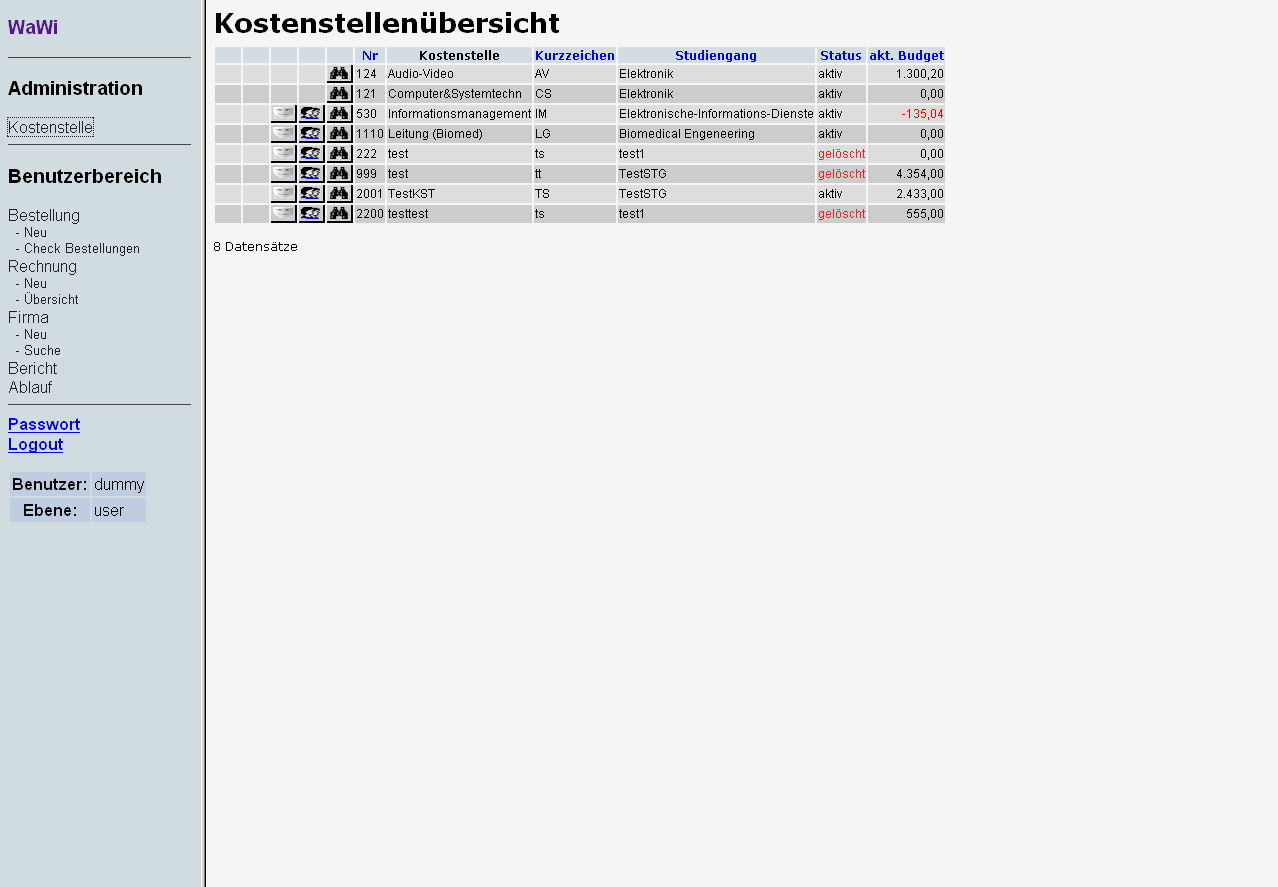
\includegraphics[width=1\textwidth]{WaWi02.png}
	\caption{Liste der Kostenstellen}
	\label{kstliste}
\end{figure}
\subsection{Aktuelle Budget�bersicht}
\label{aktbudget}
\begin{figure}
	\centering
	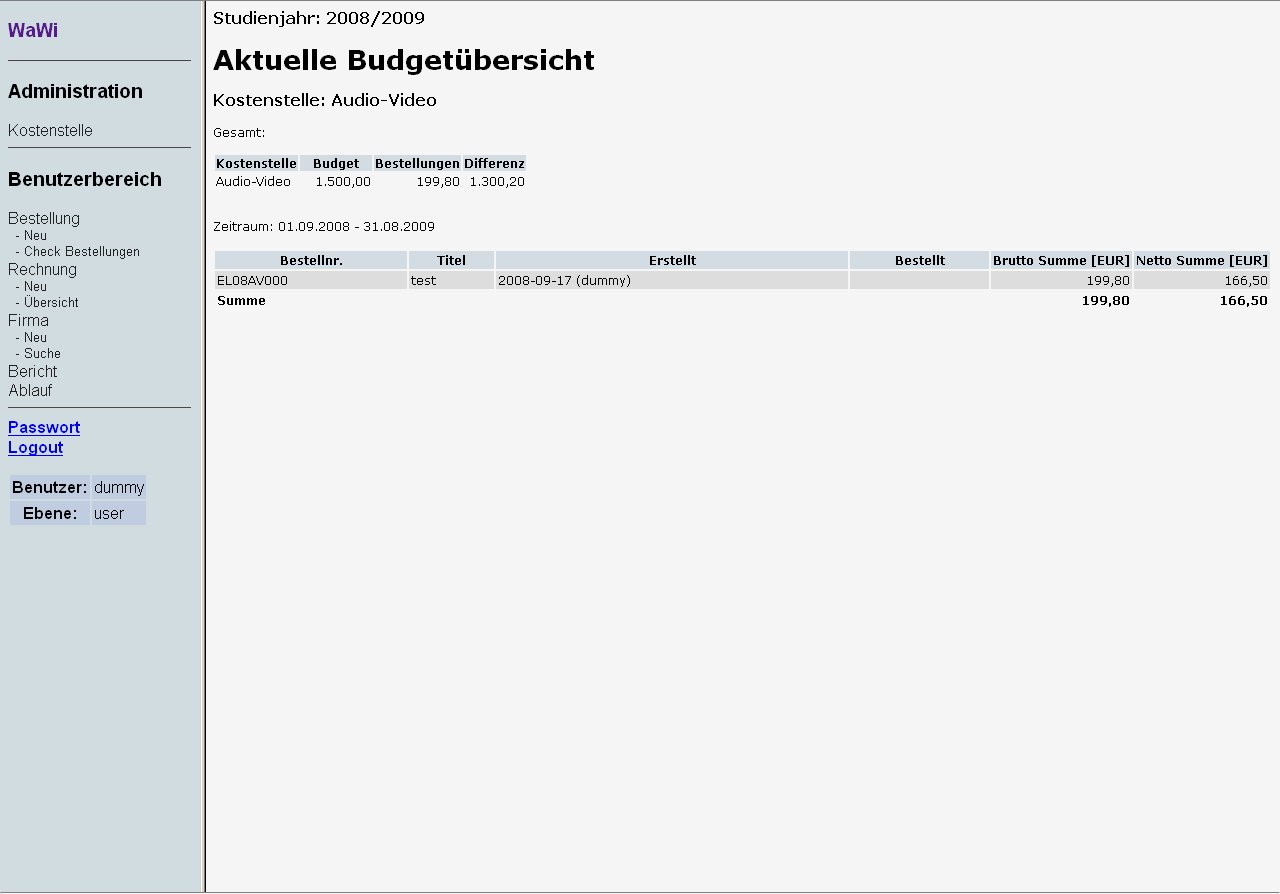
\includegraphics[width=1\textwidth]{WaWi03.png}
	\caption{Budget�bersicht}
	\label{budget}
\end{figure}
\subsection{Personalverwaltung f�r eine Kostenstelle}
\label{personal}
\begin{figure}
	\centering
	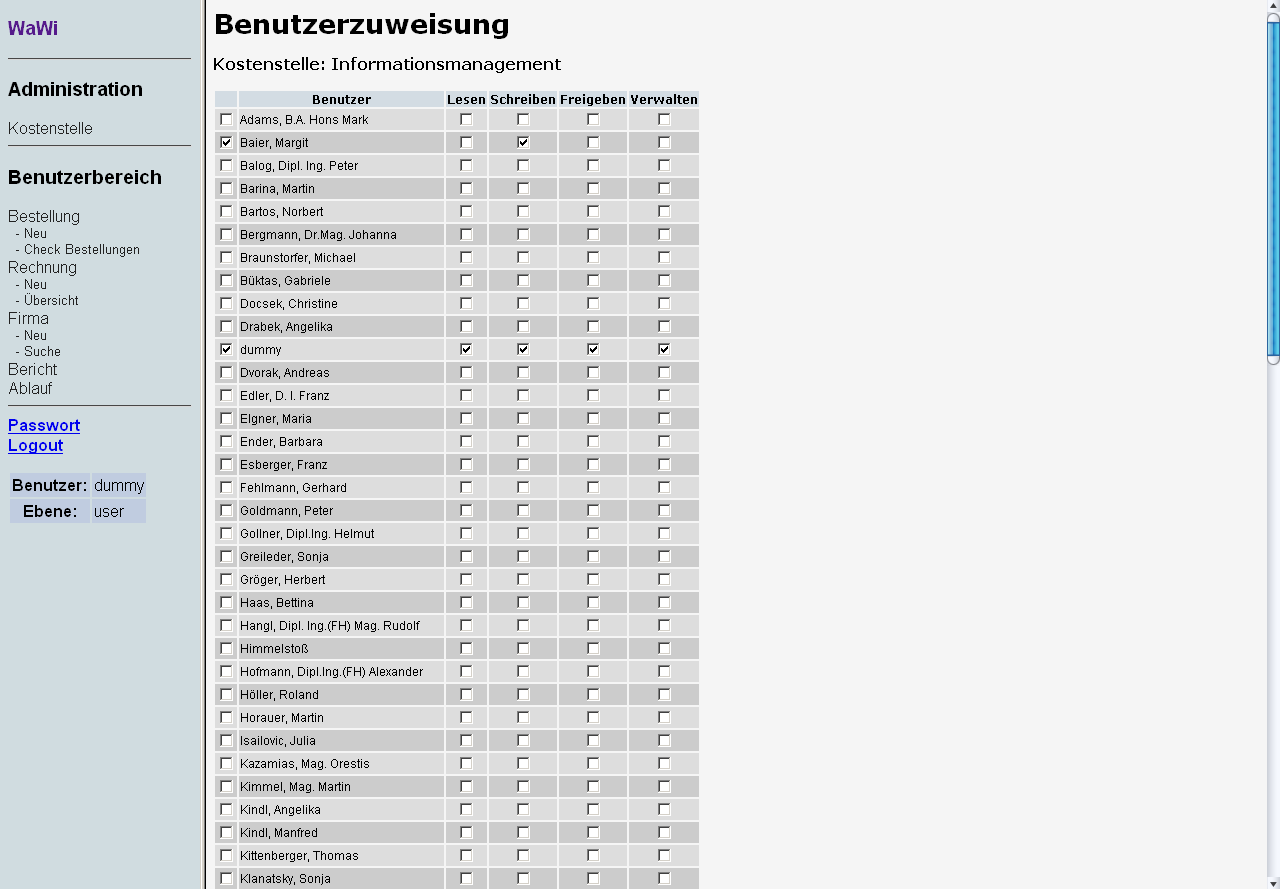
\includegraphics[width=1\textwidth]{WaWi04.png}
	\caption{Benutzerzuweisung}
	\label{kstbenutzer}
\end{figure}
